\documentclass{article}
\usepackage{graphicx,hyperref,caption,multirow}
\usepackage[spanish]{babel}
\graphicspath{{img/}}

\title{Introduccion a Packet Tracer}
\author{Luciano Nardelli  \\ {nardelli96@gmail.com}}
\date{Agosto de 2024}

\begin{document}

    \maketitle

    \section{Packet Tracer}
        
        Esta herramienta es un software de simulacion de redes desarrollado por Cisco que permite configurar,diseñar y resolver problematicas en redes de dispositivos mediante interfaces graficas intuitivas.Los tipos de archivos que se pueden guardar son:
        \begin{itemize}
        \item \textbf{Principalmente .pkt}: Red simulada en Packet Tracer y guardada, puede contente imágenes pero no cuenta con ventana de instrucciones ni puntuación de actividad.
        \item \textbf{.pka}: Es un archivo de actividad para Packet Tracer teniendo ventana de instrucciones y puntuacion
        \item \textbf{.pksz}: Es específico de Actividades asistidas en Packet Tracer que brindan apoyo a estudiantes que están trabajando para completar la actividad.
        \item \textbf{.pkz}: Se utilizaba anteriormente para incrustar imágenes y otros archivos en un archivo de Packet Tracer. Se reemplazo por .pky o .pka.
        \end{itemize}
    
        El area de trabajo de packet tracer esta compuesto por:
        \begin{itemize}
            \item \textbf{Zona de menus y barra de herramientas}: La zona de menues es el área donde se encuentran las opciones generales de todos los programas para la gestión y la configuración del software. 
            Mientras que la barra de herramientas es el area de edicion ya sea para seleccionar, inspeccionar, borrar o ajustar dispositivos; como tambien crear notas, dibujar o generar unidades de datos de protocolo simples/complejos
            
            \item \textbf{Modo de presentacion}: Permite cambiar entre esquema lógico y esquema físico a la hora de presentar los dispositivos, habitualmente se trabaja con el logico. Una breve explicacion de cada modo:
            \begin{itemize}
            \item \textbf{Logical}: Es donde se lleva a cabo mayormente el diseño y configuracion de la red, mostrando cómo los dispositivos están interconectados y cómo se configuran a nivel de software.
            \item \textbf{Physical}: Ofrece un grafico más cercano a la realidad de la coneccion de dispositivos de la red siendo muy útil para entender la implementación física y la disposición geográfica de la red.
            \end{itemize}
            
            \item \textbf{Espacio de trabajo}: Es la zona donde se situarán los dispositivos que conforman la red

            \item \textbf{Dispositivos electronicos}: Es la zona que permite seleccionar los dispositivos que van a ser incluidos en el espacio de trabajo, así como la conexión entre ellos.
            \item \textbf{Escenarios}:Sirve para realizar distintos análisis sobre una misma red.
            \item \textbf{Estado del Escenario}:Muestra las UDP(Protocolo de Datagramas de Usuario) que han intervenido en el análisis realizado para cada uno de los escenarios en los que ha operado la red
            \item \textbf{Modos de operacion}:
            \begin{itemize}
            \item \textbf{Realtime}: Ofrece una vista del comportamiento de la red como si funcionara en un entorno real. Todos sus procesos se realizan de forma instantaneamente y es ideal para configuraciones rápidas y pruebas generales.
            
            \item \textbf{Simulation}: Proporciona un control total del tiempo permitiendo observar el recorrido de los paquetes a traves de la red e ideal para analisis detallados, resolución de problemas y ver cómo funcionan los diferentes protocolos y dispositivos de una red 
            \end{itemize}
    
        \end{itemize}

    \section{Dispositivos finales}
        Son todos aquellos que se encuentran en el Network Devices
   
        Resumen de cada tipo:
        \begin{enumerate}
            \item\textbf{Router}: Conecta diferentes redes y dirige el tráfico de datos entre ellas. Tambien maneja la selección de rutas y puede realizar funciones de NAT y firewall. Los router que se pueden usar en PacketTracer son:
            \begin{itemize}
                \item\textbf{4331}:
                 \begin{itemize}
                    \item \textbf{Descripcion}:Es ideal para sucursales
                    \item \textbf{Limitacion}: Costoso y complejo de configurar.
                \end{itemize}
                \item\textbf{4321}: 
                 \begin{itemize}
                    \item \textbf{Descripcion}:Para pequeñas sucursales.
                    \item \textbf{Limitacion}: Menor capacidad que el 4331
                \end{itemize}
                \item\textbf{1941}:
                 \begin{itemize}
                    \item \textbf{Descripcion}: Adecuado para pequeñas empresas
                    \item \textbf{Limitacion}: Menos potente que los modelos más nuevos.
                \end{itemize}
                \item\textbf{2901}:
                 \begin{itemize}
                    \item \textbf{Descripcion}:Ofrece buen rendimiento.
                    \item \textbf{Limitacion}: Menos capacidad que la serie 4000.
                \end{itemize}
                \item\textbf{2911}:
                 \begin{itemize}
                    \item \textbf{Descripcion}: Variante mejorada del 2901 con más interfaces.
                    \item \textbf{Limitacion}: Esta limitado frente a la serie 4000
                \end{itemize}
                \item\textbf{819IOX}:
                 \begin{itemize}
                    \item \textbf{Descripcion}: Router para IoT y redes móviles.
                    \item \textbf{Limitacion}:  Limitado en expansión y procesamiento.
                \end{itemize}
                \item\textbf{819HGW}:
                 \begin{itemize}
                    \item \textbf{Descripcion}: Router para IoT con conectividad celular.
                    \item \textbf{Limitacion}: Similar al 819IOX, específico para aplicaciones IoT.
                \end{itemize}
                \item\textbf{829}:
                 \begin{itemize}
                    \item \textbf{Descripcion}: Router robusto para aplicaciones IoT y móviles.
                    \item \textbf{Limitacion}: Enfocado en aplicaciones específicas, menos versátil.
                \end{itemize}
                \item\textbf{1240}:
                 \begin{itemize}
                    \item \textbf{Descripcion}: Router inalámbrico para redes LAN empresariales
                    \item \textbf{Limitacion}: Menos capacidad comparado con routers más modernos.
                \end{itemize}
                \item\textbf{Pt-Router}:
                 \begin{itemize}
                    \item \textbf{Descripcion}: Router genérico para prácticas en Packet Tracer
                    \item \textbf{Limitacion}: Funcionalidades básicas, no refleja hardware real.
                \end{itemize}
                \item\textbf{Pt-Empy}:
                 \begin{itemize}
                    \item \textbf{Descripcion}: Chasis de router vacío para personalización.
                    \item \textbf{Limitacion}:  Requiere configuración manual de módulos.
                \end{itemize}
                \item\textbf{1841}:
                 \begin{itemize}
                    \item \textbf{Descripcion}:  Router básico de la serie 1800.
                    \item \textbf{Limitacion}: Capacidad de expansión limitada.
                \end{itemize}
                \item\textbf{2620XM}:
                 \begin{itemize}
                    \item \textbf{Descripcion}: Router antiguo de la serie 2600.
                    \item \textbf{Limitacion}: Soporte limitado para tecnologías actuales.
                \end{itemize}
                \item\textbf{2621XM}:
                 \begin{itemize}
                    \item \textbf{Descripcion}: Variante del 2620XM con más interfaces.
                    \item \textbf{Limitacion}: Similar al 2620XM, obsoleto para redes modernas
                \end{itemize}
                \item\textbf{2811}:
                 \begin{itemize}
                    \item \textbf{Descripcion}: Router de la serie 2800, adecuado para redes medianas.
                    \item \textbf{Limitacion}: Menos eficiente que los routers más recientes.
                \end{itemize}
            \end{itemize}
            
            \item\textbf{Switcher}: conecta múltiples dispositivos dentro de la misma red local (LAN), permitiendo la comunicación entre ellos. A diferencia de un hub, envía datos solo al dispositivo específico que lo necesita, mejorando la eficiencia de la red.
            \begin{itemize}
                \item \textbf{2960}:
                \begin{itemize}
                    \item \textbf{Descripcion}: Switch de capa 2, ideal para redes pequeñas y medianas. Soporta funciones básicas de switching y seguridad.
                    \item \textbf{Limitacion}: No tiene capacidades avanzadas de capa 3 y es menos flexible en entornos complejos.
                \end{itemize}
                \item \textbf{Pt-Switch}:
                \begin{itemize}
                    \item \textbf{Descripcion}: Switch genérico en Packet Tracer para configuraciones básicas.
                    \item \textbf{Limitacion}: Funcionalidades limitadas y no representa un modelo real específico.
                \end{itemize}
                \item \textbf{Pt-Empy}:
                \begin{itemize}
                    \item \textbf{Descripcion}: Chasis de switch vacío que permite añadir módulos personalizados en Packet Tracer.
                    \item \textbf{Limitacion}: Requiere conocimiento avanzado para configurar adecuadamente los módulos.
                \end{itemize}
                \item \textbf{3560 24ps}:
                \begin{itemize}
                    \item \textbf{Descripcion}: Switch de capa 3 con 24 puertos, adecuado para redes empresariales con capacidades de enrutamiento.
                    \item \textbf{Limitacion}: Puede ser costoso y complejo para redes pequeñas.
                \end{itemize}
                \item \textbf{3650 24ps}:
                \begin{itemize}
                    \item \textbf{Descripcion}: Switch de capa 3 con mayor rendimiento y soporte para PoE, adecuado para redes con alta demanda de tráfico.
                    \item \textbf{Limitacion}:  Más caro y con mayor consumo de energía, lo que lo hace menos eficiente para redes pequeñas.
                \end{itemize}
                \item \textbf{IE 2000}:
                \begin{itemize}
                    \item \textbf{Descripcion}: Switch industrial para entornos robustos, con características de alta disponibilidad y seguridad.
                    \item \textbf{Limitacion}: Enfocado en entornos industriales, no es adecuado para oficinas o entornos convencionales.
                \end{itemize}
             \item \textbf{PT Bridge}:
                \begin{itemize}
                    \item \textbf{Descripcion}:  Dispositivo en Packet Tracer que actúa como un puente, permitiendo la conexión de diferentes segmentos de red.
                    \item \textbf{Limitacion}: Funcionalidad limitada en comparación con switches y routers reales, ya que no ofrece capacidades avanzadas de red.
                \end{itemize}
                \item \textbf{2950-24}:
                \begin{itemize}
                    \item \textbf{Descripcion}: Switch de capa 2 con 24 puertos, adecuado para redes básicas.
                    \item \textbf{Limitacion}: Sin soporte para enrutamiento, limitado a funciones básicas de switching.
                \end{itemize}
                \item \textbf{2950DT}:
                \begin{itemize}
                    \item \textbf{Descripcion}: Variante del 2950 con más características de seguridad y administración.
                    \item \textbf{Limitacion}: Aún limitado a capa 2 y no soporta funciones avanzadas de capa 3.
                \end{itemize}
            \end{itemize}
            \item\textbf{Hub}: Conecta múltiples dispositivos en una red local. Reenvía los datos recibidos a todos los dispositivos conectados generando tráfico innecesario en la red.  
            \item\textbf{Wireless Devices}: Permiten que dispositivos se conecten a la red sin necesidad de cables. Estos extienden la cobertura de la red mediante señales Wi-Fi.  
            \item\textbf{Security}: Dispositivos como firewalls y sistemas de prevención de intrusiones que protegen la red al controlar el tráfico y detectar amenazas.  
            \item\textbf{WAN Emulation}: Simula redes de área amplia (WAN) para probar el rendimiento y comportamiento de las redes bajo diversas condiciones. 
        \end{enumerate}
        

    \section{Dispositivos de red}
       Algunos EndDevices son:
       \begin{itemize}
           \item\textbf{PC}:
            \begin{itemize}
                \item\textbf{Modulos}:
                \begin{itemize}
                    \item\textbf{WMP300N}: Proporciona una interfaz inalámbrica de 2,4 GHz adecuada para la conexión a redes inalámbricas. El módulo admite protocolos que utilizan Ethernet para el acceso LAN.
                    \item\textbf{PT-HOST-NM-1AM}: Cuenta con conectores duales RJ-11, que se utilizan para conexiones de servicio telefónico básico. El WIC-1AM utiliza un puerto para la conexión a una línea telefónica estándar y el otro puerto se puede conectar a un teléfono analógico básico para usarlo cuando el módem está inactivo.
                    \item\textbf{PT-HOST-NM-1CE}: Cuenta con un único puerto Ethernet que puede conectar una red troncal LAN que también puede admitir seis conexiones PRI para agregar líneas ISDN o 24 puertos síncronos/asincrónicos.
                    \item\textbf{PT-HOST-NM-1CFE}: Proporciona una interfaz Fast-Ethernet para usar con medios de cobre. Ideales para una amplia gama de aplicaciones LAN, los módulos de red Fast Ethernet admiten muchas funciones y estándares de interconexión en red. Los módulos de red de un solo puerto ofrecen Ethernet 10/100BaseTX o 100BaseFX con detección automática. La versión TX (cobre) admite la implementación de LAN virtual (VLAN)
                    \item\textbf{PT-HOST-NM-1CGE}: Proporciona conectividad de cobre Gigabit Ethernet para enrutadores de acceso. El módulo es compatible con los enrutadores de las series Cisco 2691, Cisco 3660, Cisco 3725 y Cisco 3745. Este módulo de red tiene una ranura de convertidor de interfaz gigabit (GBIC) para transportar cualquier GBIC Cisco óptico o de cobre estándar.
                    \item\textbf{PT-HOST-NM-1FFE}: Proporciona una interfaz Fast-Ethernet para usar con medios de fibra. Ideales para una amplia gama de aplicaciones LAN, los módulos de red Fast Ethernet admiten muchas funciones y estándares de interconexión en red. Los módulos de red de un solo puerto ofrecen Ethernet 10/100BaseTX o 100BaseFX con detección automática.
                    \item\textbf{PT-HOST-NM-1FGE}: El módulo de red Cisco Gigabit Ethernet de un solo puerto proporciona conectividad óptica Gigabit Ethernet para enrutadores de acceso. El módulo es compatible con los enrutadores de las series Cisco 2691, Cisco 3660, Cisco 3725 y Cisco 3745. Este módulo de red tiene una ranura de convertidor de interfaz gigabit (GBIC) para transportar cualquier GBIC Cisco óptico o de cobre estándar.
                    \item\textbf{PT-HOST-NM-1W}: Proporciona una interfaz inalámbrica de 2,4 GHz adecuada para la conexión a redes inalámbricas. El módulo admite protocolos que utilizan Ethernet para el acceso LAN. 
                    \item\textbf{PT-HOST-NM-1W-A}: Proporciona una interfaz inalámbrica de 5 GHz adecuada para la conexión a redes inalámbricas 802.11a. El módulo admite protocolos que utilizan Ethernet para el acceso LAN.
                    \item\textbf{PT-HOST-NM-1W-AC}: Proporciona una interfaz inalámbrica de 5 GHz adecuada para la conexión a redes inalámbricas 802.11ac o 802.11b/g/n en la banda de 2,4 GHz. El módulo admite protocolos que utilizan Ethernet para el acceso LAN.
                    \item\textbf{PT-HOST-NM-3G/4G}: Proporciona una interfaz celular adecuada para la conexión a redes 3G/4G.
                    \item\textbf{PT-HOST-NM-COVER}: La placa de cubierta proporciona protección a los componentes electrónicos internos. También ayuda a mantener una refrigeración adecuada al normalizar el flujo de aire.
 
                    \item\textbf{PT-HEADPHONE}: Los auriculares permiten al usuario escuchar música y sonidos desde la computadora.
                    \item\textbf{PT-MiCROPHONE}: El micrófono permite que la computadora grabe sonido.
                \end{itemize}
                \item\textbf{Firmware}: Los PCs en Packet Tracer incluyen un firmware básico que permite ejecutar configuraciones de red, acceso a CLI, y algunas aplicaciones predeterminadas como un navegador web y un terminal de comandos.
                Las cosas que tienen en desktop son:
                IP Configuration, Dial-up, Terminal, Command Prompt, Web browser, PC Wireless, VPN,Traffic Generator, MIB Browser, Cisco IP Communicator,Email, PPPoE Dialer, Text Editor,Firewall IPv6 Firewall, Netflow Collector, IoX IDE, TFTP Service, Telnet / SSH Client, Bluetooth, IoT Monitor, Iot IDE y User Apps Manager
                \item\textbf{Tarjetas}:
                \begin{itemize}
                    \item\textbf{NIC Ethernet}: Para conectividad básica por cable.
                    \item\textbf{NIC inalámbrica}: Para Wi-Fi.
                    \item\textbf{Interfaz Serial}: Para conexiones seriales en redes más avanzadas.
                    \item\textbf{Módulo de expansión}: Para añadir más puertos o funcionalidades específicas.
                \end{itemize}
            \end{itemize}
           \item\textbf{Laptops}: 
           \begin{itemize}
                \item\textbf{Modulos}: Son los mismos modulos que PC solo que reemplaza el HOST por LAPTOP y no cuentan con un NM-COVER 
                \item\textbf{Firmware}: Tienen un firmware similar al de los PCs.
                Las cosas que tienen en desktop son:
                IP Configuration, Dial-up, Terminal, Command Prompt, Web browser, PC Wireless, VPN,Traffic Generator, MIB Browser, Cisco IP Communicator,Email, PPPoE Dialer, Text Editor,Firewall IPv6 Firewall, Netflow Collector, IoX IDE, TFTP Service, Telnet / SSH Client, Bluetooth, IoT Monitor, Iot IDE y User Apps Manager
                \item\textbf{Tarjetas}: Cuentan con NIC inalambricos,NIC Ethernet y modulos USB
            \end{itemize}
           \item\textbf{Servidor}:
           \begin{itemize}
                \item\textbf{Modulos}: Cuenta con algunos Modulos del pc tales como: WNP300N, PT-HOST-NM-1CE, PT-HOST-NM-1CFE, PT-HOST-NM-1CGE, PT-HOST-NM-1FFE, PT-HOST-NM-1FGE, PT-HOST-NM-1W,PT-HOST-NM-1W, PT-HOST-NM-1W-A, PT-HOST-NM-1W-AC, PT-HOST-NM-3G/4G y PT-HOST-NM-COVER
                \item\textbf{Firmware}: Los servidores pueden expandirse con múltiples NICs, interfaces seriales, y módulos de almacenamiento adicionales para simular entornos complejos.
                Las cosas que tienen en desktop son:
                IP Configuration,Terminal, Command Prompt, Web browser, PC Wireless, VPN,AAAAccounting,Traffic Generator, MIB Browser, Cisco IP Communicator,Email, PPPoE Dialer, Text Editor,Firewall IPv6 Firewall, Netflow Collector, IoX IDE, TFTP Service, Telnet / SSH Client, Bluetooth, IoT Monitor, Iot IDE y User Apps Manager
                \item\textbf{Tarjetas}:
                \begin{itemize}
                    \item\textbf{Múltiples NIC Ethernet}: Para configurar diferentes redes o servicios. 
                    \item\textbf{Tarjetas Seriales}: Para conexiones avanzadas 
                    \item\textbf{Módulos de expansión}: Incluyen almacenamiento adicional y puertos adicionales para redes.
                \end{itemize}
            \end{itemize}
           \item\textbf{Printer}
           \begin{itemize}
                \item\textbf{Modulos}: Cuenta con los mismos modulos que el servidor
                \item\textbf{Firmware}: Tienen un firmware basico que los permite conectarse a la red y simular funcion impresora
                \item\textbf{Tarjetas}: Permite NIC Ethernet y NIC inalámbrica
            \end{itemize}
       \end{itemize}
    \section{Cableado}
       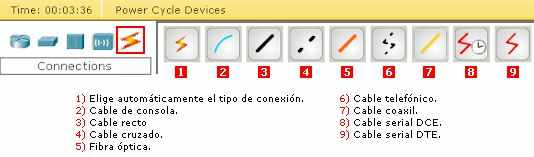
\includegraphics[width=\textwidth]{img/Cables Packet Tracer.PNG}
        Tipos de Cables:
        
        \begin{itemize}
            \item\textbf{Automatically Choose Connection Type}: 
                \begin{itemize}
                    \item\textbf{Descripcion}:  Permite que los dispositivos ajusten automáticamente la configuración de las conexiones de los cables para funcionar correctamente con cualquier tipo de cable de cobre (straight-through o crossover).
                    \item\textbf{Limitaciones}:
                    Requiere que los dispositivos conectados tengan soporte para la función automatica
                \end{itemize}   
            \item\textbf{Console}: 
                \begin{itemize}
                    \item\textbf{Descripcion}: Utilizado para la configuración inicial de dispositivos de red, conectando un PC a la consola de router o switch.
                    \item\textbf{Limitaciones}: 
                    No transporta datos de red, solo se usa para la configuración directa a través de la línea de comandos.
                \end{itemize} 
            \item\textbf{Copper Straight-Through}: 
                \begin{itemize}
                    \item\textbf{Descripcion}:
                    Utilizado para conectar dispositivos diferentes, como un switch a un router, un PC a un switch, o un router a un hub.
                    \item\textbf{Limitaciones}:
                    No puede usarse para conectar dispositivos del mismo tipo, como switch a switch o router a router.
                \end{itemize} 
            \item\textbf{Copper Crossover}: 
                \begin{itemize}
                    \item\textbf{Descripcion}:
                    Usado para conectar dispositivos del mismo tipo, como switch a switch, router a router, o PC a PC.
                    \item\textbf{Limitaciones}:
                    No adecuado para conexiones entre dispositivos diferentes, aunque muchos equipos modernos tienen puertos Automatic Conexion que pueden ajustar automáticamente el tipo de cable
                \end{itemize} 
            \item\textbf{Fiber}: 
                \begin{itemize}
                    \item\textbf{Descripcion}:
                    Utilizado para conexiones de alta velocidad y largas distancias, generalmente entre switches o routers 
                    \item\textbf{Limitaciones}:
                    Más caro y frágil que los cables de cobre, y requiere puertos específicos en los dispositivos.
                \end{itemize} 
            \item\textbf{Phone}: 
                \begin{itemize}
                    \item\textbf{Descripcion}:
                    Utilizado para conectar dispositivos de telefonía, como teléfonos analógicos,etc
                    \item\textbf{Limitaciones}:
                    Limitado a conexiones de baja velocidad para voz.No adecuado para la transmisión de datos de red.Solo se usa en la emulación de redes de telefonía.
                \end{itemize} 
            \item\textbf{Coaxial}:
                \begin{itemize}
                    \item\textbf{Descripcion}:
                    Utilizado en tecnologías de red más antiguas, como redes Ethernet de banda base o sistemas de televisión por cable.
                    \item\textbf{Limitaciones}:
                    Raramente utilizado en redes modernas debido a su menor capacidad de transmisión en comparación con otras tecnologías.
                \end{itemize} 
            \item\textbf{Serial DCE}: 
                \begin{itemize}
                    \item\textbf{Descripcion}:
                    Conecta interfaces seriales entre routers, con un extremo definido como DCE, que provee la tasa de reloj para la comunicación.

                    \item\textbf{Limitaciones}:
                    Se requiere para configurar la tasa de reloj en la interfaz DCE, lo cual es esencial para la comunicación.Limitado a conexiones WAN de baja velocidad en comparación con otros métodos más modernos como Ethernet.
                \end{itemize} 
            \item\textbf{Serial DTE}: 
                \begin{itemize}
                    \item\textbf{Descripcion}:
                    Conecta interfaces seriales entre routers, con un extremo definido como DTE, que recibe la tasa de reloj del DCE.
                    \item\textbf{Limitaciones}:
                    Depende del DCE para la configuración de la tasa de reloj. Limitado a conexiones WAN y es menos común en redes modernas.
                \end{itemize} 
            \item\textbf{Octal}: 
                \begin{itemize}
                    \item\textbf{Descripcion}:
                    Un cable especial que conecta un router a múltiples dispositivos seriales a través de una interfaz de consola. Es un cable con múltiples salidas.
                    \item\textbf{Limitaciones}:
                    Solo es útil en entornos que requieren la conexión y configuración de múltiples dispositivos desde un solo puerto del router. No transporta datos de red, solo se usa para la configuración.
                \end{itemize} 
            \item\textbf{IoT Custom}:
                \begin{itemize}
                    \item\textbf{Descripcion}:
                    Un cable genérico utilizado en conexiones personalizadas entre dispositivos IoT en Packet Tracer
                    \item\textbf{Limitaciones}:
                    Es específico para el entorno de simulación y no refleja un cable físico estándar en redes reales. Su funcionalidad está limitada al entorno de IoT de Packet Tracer, y no se puede usar para conexiones regulares de red.
                \end{itemize} 
            \item\textbf{USB}: 
                \begin{itemize}
                    \item\textbf{Descripcion}:
                    Conecta dispositivos periféricos como impresoras, cámaras, y otros equipos USB a PCs o routers.
                    \item\textbf{Limitaciones}:
                    La longitud máxima de un cable USB estándar es de 5 metros sin usar repetidores.
                    Principalmente para la conexión de dispositivos periféricos, no diseñado para conexiones de red largas o de alta velocidad
                \end{itemize} 
        \end{itemize}
        
    \section{Referencias}
        \begin{itemize}
            \item Youtube
                \begin{itemize} 
                \item \href{https://www.youtube.com/watch?v=lso8MPblUZY&list=PLINy58Bvq5_IV5dhYqGy500vSTCIHUkS1&index=4}{[II] CISCO PACKET TRACER (La serie): Explorando la Interfaz, Configuración y Conexiones}
                \end{itemize}
            \item Documentacion Oficial
                \begin{itemize} 
                \item \href{https://skillsforall.com/es/course/getting-started-cisco-packet-tracer?courseLang=es-XL}{Introduccion a Cisco Packet}            
                \end{itemize}
            \item Otras paginas
            \begin{itemize} 
                \item \href{https://ipcisco.com/lesson/network-devices-2/}{Network Devices}
                \item  \href{https://ccnatutorials.in/packet-tracer/types-of-cables-in-packet-tracer/}{Tipos de Cables in Packet Tracer}
                \item \href{ https://learningnetwork.cisco.com/s/article/el-software-de-simulacion-cisco-packet-tracer}{Introduccion a Cisco Packet}
            \end{itemize}
            \item Repositorio \href{https://github.com/nardo96hub/Redes1-Entregas/tree/main/Introduccion%20Packet%20Tracer}{Github} del codigo latex
            
        \end{itemize}

    \section{Experimento}
         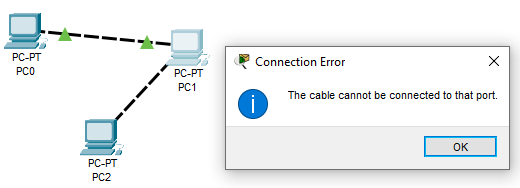
\includegraphics[width=\textwidth]{img/Experimento.PNG}
         En la imagen se puede observar que no se pueden conectar 3 pc si 2 de ellas se comunican entre si. Para poder conseguir eso es necesario que las 3 se conecten a un switch como se observa abajo
        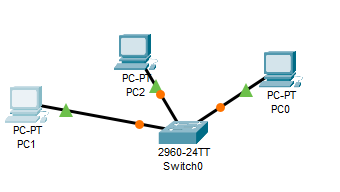
\includegraphics[width=\textwidth]{img/Conectar PCS.PNG}
    \pagestyle{plain}
\end{document}